\documentclass[a4paper]{article}

\usepackage[utf8]{inputenc}
\usepackage[L7x]{fontenc}
\usepackage[lithuanian]{babel}
\usepackage{lmodern}
\usepackage{hyperref}
\usepackage{amsmath} %systems, equations and so on
\usepackage{framed}
\usepackage{graphicx}
\usepackage{mathtools}

\usepackage{geometry}
 \geometry{
 a4paper,
 right=20mm,
 left=20mm,
 top=20mm,
bottom=20mm,
 }

\begin{document}

\makeatletter %creating a special kind of braces
\newenvironment{sqcases}{%
  \matrix@check\sqcases\env@sqcases
}{%
  \endarray\right.%
}
\def\env@sqcases{%
  \let\@ifnextchar\new@ifnextchar
  \left\lbrack
  \def\arraystretch{1.2}%
  \array{@{}l@{\quad}l@{}}%
}
\makeatother

\section{}

Hello.  Night Simon is coming silently into the room. \href{portretas.jpg}{\textbf{Hi, Simon!}}
\section{}
Press his bolded name. Can you see him. Well, it woud be great to consider all the things that can happen:

$\begin{sqcases}
\text {You can see him} \Rightarrow \text{He is \href{http://www.soundjay.com/human/sounds/applause-01.mp3}{\textbf{clapping}} for you!} \\
\text {You can't see him} \Rightarrow 
\begin{sqcases}
\text {You don't wish to see him} \Rightarrow \text{Please, turn off your computer and go out to breathe a fresh air} \\
\text {You wish to see him} \Rightarrow 
\begin{aligned}[c]
& \text{Try to open this file via \href{https://get.adobe.com/reader/}{\textbf{Acrobat Reader}}}\\
& \text{and follow the instructions in the \href{README.txt}{\textbf{README}} file}
\end{aligned}
\end{sqcases}
\end{sqcases}$

\section{}

If Simon is in a good mood, he will tell you a story.

\begin{framed}
\textit{Boys requires TIME and MONEY:} 

$BOYS=TIME \cdot MONEY$

\textit{TIME is MONEY thus}

$BOYS=MONEY \cdot MONEY=MONEY^2$

\textit{The MONEY are ROOTS of evil thus  }

$BOYS=\Big(\sqrt{EVIL}\Big)^2=EVIL$
\end{framed}

Don't worry if it sounds like some kind of bullshit sometimes. \href{mailto:simonas.mamaitis@gmail.com}{\textbf{You can complain him}} about that.

\section{}

If Simon is in a bad mood he looks \href{https://www.facebook.com/photo.php?fbid=1791779717765839&set=a.1720498398227305.1073741828.100008014839713&type=3&theater}{\textbf{terribly}}

\section{}

Simon is not lonely. He like a company of his friends: \href{http://pastebin.com/v9xYFc3i}{\textbf{Diana}}, \href{http://pastebin.com/yqhNy1UR}{\textbf{Caroline}} and \href{http://pastebin.com/hjv7bP2T}{\textbf{Grethe}}.

\section{}

When Simon works with music he creates an artwork of  \href{https://soundcloud.com/naktinis-saimonas/simon-production}{\textbf{sound}} from mathematical expressions

\section{}

When Simon works with mathematics he creates a complicated \href{run:diskr.pdf}{\textbf{article}} with many many symbols.

\section{}

\href{http://www.youtube.com/watch?v=7WwLT32_VAk&t=23m30s}{\textbf{Adieu!}}

\begin{center}
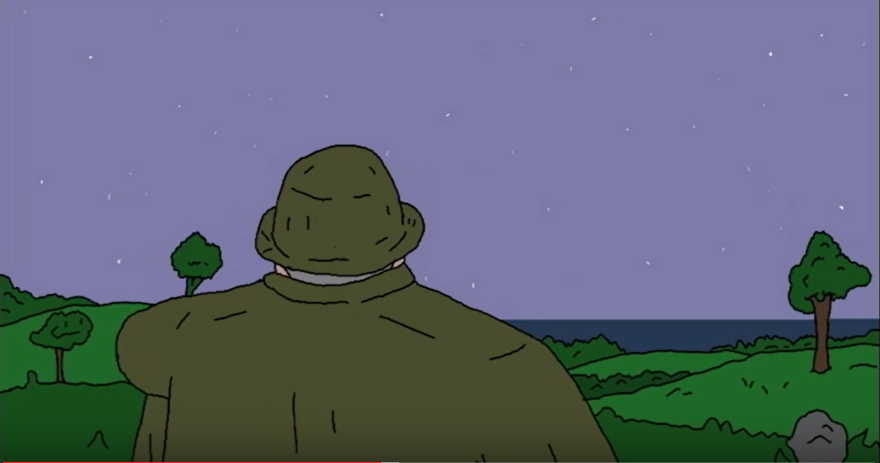
\includegraphics[width=80mm]{fairy.png}
\end{center}
\end{document}